\documentclass[10pt,letterpaper]{article}
\usepackage[margin=.82in]{geometry}
\usepackage[T1]{fontenc}\usepackage{lmodern,graphicx,booktabs,amsmath,xcolor,hyperref,xurl,caption,fancyhdr}
\hypersetup{colorlinks=true,urlcolor=teal,linkcolor=teal,pdftitle={Test false rejections before using an ECG quality gate},pdfauthor={James Jean}}
\pagestyle{fancy}\fancyhf{}\fancyhead[L]{\small ECG quality gate / Study 39}\fancyhead[R]{\small Independent negative-result benchmark}\fancyfoot[C]{\thepage}
\setlength{\headheight}{14pt}\setlength{\parindent}{0pt}\setlength{\parskip}{6pt}\captionsetup{font=small,labelfont=bf,hypcap=false}
\begin{document}
{\small\color{teal} SIGNAL QUALITY / CHECK THE COST OF REJECTION\par}
\vspace{7pt}{\LARGE\bfseries Test false rejections before\par using an ECG quality gate\par}
\vspace{7pt}James Jean \hfill 30 October 2026

\textbf{Decision.} A rule that catches added ECG noise can still reject too much source-clean signal. Before using such a rule, measure both outcomes on later windows and another recording. A short clean calibration period does not guarantee a stable rejection rate.

\textbf{Measured finding.} All three authored candidate gates fail the declared 5\% source-clean false-rejection limit. Even the least aggressive flags 58 of 150 later source-clean development windows (38.7\%); the most aggressive flags 52.0\%. The fixed selection rule therefore keeps the accept-all fallback. This means that no quality gate is eligible under this exercise's assumptions; it does not certify any window as clinically clean.

\begin{center}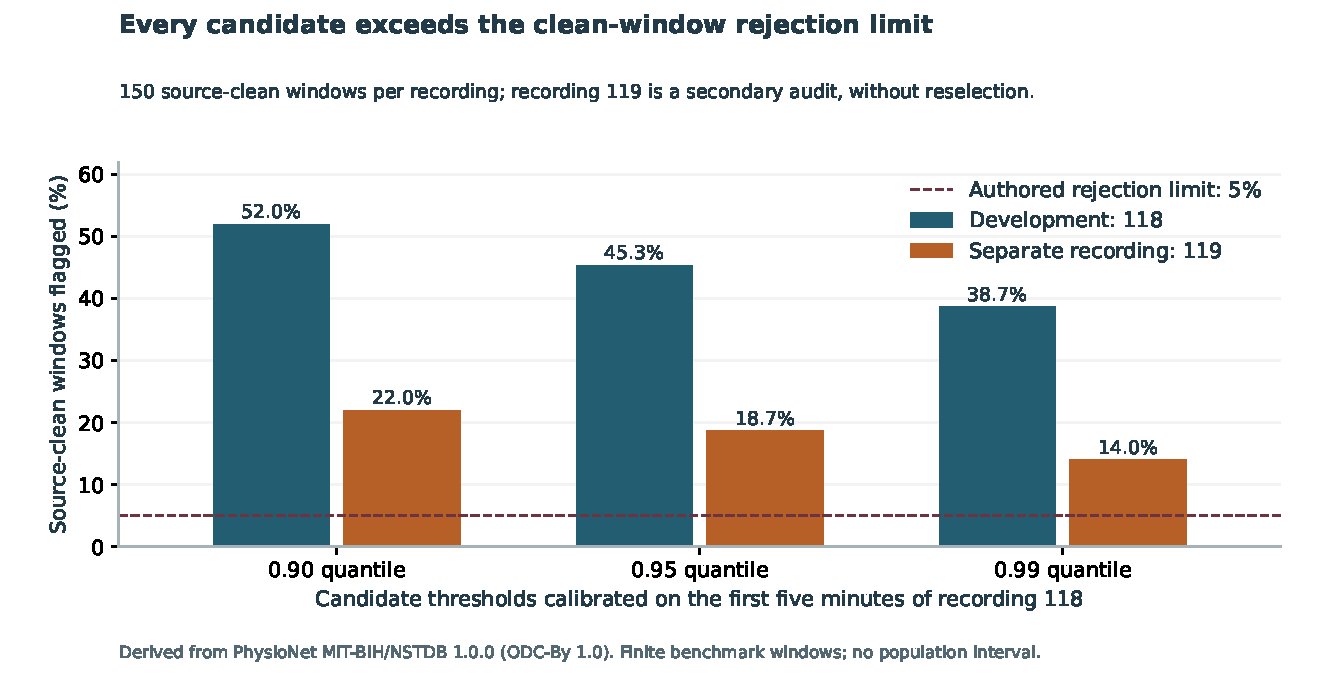
\includegraphics[width=\linewidth]{images/clean_window_rejections.pdf}\end{center}
\captionof{figure}{Both the development and separate-recording results retain the failed rejection constraint. Each bar uses its recording's source-clean control windows. Recording 119 is a secondary diagnostic of already rejected candidates; there is no later reselection. The dashed limit is an authored demonstration assumption, not a validated clinical operating requirement.}

\textbf{Separate-recording check.} The least aggressive rejected candidate flags 21 of 150 source-clean windows (14.0\%) on the other recording; all three span 14.0--22.0\%. This secondary result does not rescue their development failure. The frozen fallback produces no noise-detection improvement.

\textbf{Practical recommendation.} Do not deploy these candidate gates from this evidence. Keep the complete failure table, test source-clean rejection alongside noise detection, and obtain representative recordings and expert quality judgments before choosing an operational rule. No downstream clinical prediction, device comparison, alarm reduction or patient benefit is measured here.
\newpage
\section*{1. Fixed public sources, with a source-binding correction}
The open-access MIT-BIH Noise Stress Test Database 1.0.0 supplies six calibrated electrode-motion noise variants of each of two source ECG recordings, 118 and 119. The source-clean recordings come from the MIT-BIH Arrhythmia Database 1.0.0. This is 14 fixed waveform records in total. The acquisition preserves 37 files, including headers, published checksum inventories and source/format/rights pages. Every waveform/header SHA-256 agrees with the publisher inventory. Original waveforms, header comments and annotations remain outside Git.

Both sources use the Open Data Commons Attribution License 1.0. The public package contains derived features, public record identifiers, sanitized encoding metadata and new calculations. It contains no demographic or medication comments, private clinical records, protected PhysioNet datasets or third-party papers. The authored-code license does not relicense source rights. Contains information from the MIT-BIH and Noise Stress Test databases, made available under ODC Attribution 1.0; the source and license links appear on the final page.

\textbf{Encoding and source shape.} A vectorized reader supports the native multiplexed 212 and little-endian 16-bit formats. It checks signal count, sampling rate, length, initial values, physical gain/baseline and signed native checksums. Independent WFDB decoding agrees on all 18,200,000 digital samples and their physical conversions. Both channels are checked; only signal 0, MLII, enters the feature study.

The first clean-interval check incorrectly required equality of absolute voltages after native physical conversion. It failed before feature computation. The publisher's NST documentation specifies additive offsets recalculated at noise transitions to prevent step changes. Diagnostic comparisons confirmed constant offsets within clean segments. The corrected, committed source check requires matching gains and stress-minus-original digital values constant to within one ADC unit in each clean segment and channel. All 8,812,800 clean-interval cells pass. No time shift, scale fit, filtering or waveform correction is applied. The failed check, diagnostic and original protocol are retained; absolute-voltage equality is not claimed.

\textbf{Complete window projection.} Each recording contributes 648 derived feature rows: 180 source-clean windows and six groups of 78 added-noise windows. Windows last ten seconds at 360 Hz. The first thirty minutes are used; the final extra tail is excluded by design. The source's initial five minutes are clean, followed by alternating two-minute noisy and clean segments. Duplicate clean segments from six SNR variants are checked for source shape but are not multiplied into independent negative observations.

\begin{center}\begin{tabular}{@{}lr@{}}\toprule
Development role on recording 118 & Windows\\\midrule
Initial source-clean calibration & 30\\
Later source-clean controls & 150\\
Each added-noise stratum & 78\\
\bottomrule\end{tabular}\end{center}

Primary noise positives pool the fixed -6, 0 and 6 dB conditions. Other noise levels are secondary strata, not clinically acceptable negatives. The labels describe a source-generated stress condition, not an expert clinical acceptability judgment. Recording 119 never calibrates thresholds.
\newpage
\section*{2. Simple features and a search that fails its constraint}
For a complete 3,600-sample physical-mV window, write $\bar x$ for its mean and $V$ for its centered mean-square value. Flat, nonfinite or malformed input is unavailable. Define two dimensionless authored features:
\[
 V={1\over3600}\sum_{i=1}^{3600}(x_i-\bar x)^2,\qquad
 H={\frac1{3599}\sum_{i=1}^{3599}(x_{i+1}-x_i)^2\over V},
\]
\[
 B={\frac1{10}\sum_{j=1}^{10}(\bar x_j-\bar x)^2\over V},
\]
where $\bar x_j$ is the mean of the $j$th nonoverlapping one-second block. $H$ measures adjacent-difference energy relative to centered energy; $B$ measures slow block-mean variation. Window and block lengths are fixed engineering choices, not tuned clinical frequency cutoffs. A new window requires no reference ECG, annotations, future windows or inference-time label.

Each candidate sets its two thresholds to nearest-rank quantiles of the first thirty source-clean development windows. A window is flagged if either feature is strictly above its threshold. The finite grid and the full fitted values are retained:
\begin{center}\begin{tabular}{@{}lrr@{}}\toprule
Calibration quantile & $B$ threshold & $H$ threshold\\\midrule
0.90 & 0.109284 & 0.030673 \\
0.95 & 0.123295 & 0.031517 \\
0.99 & 0.217040 & 0.031776 \\
\bottomrule\end{tabular}\end{center}

Select only a nonbaseline candidate with at most 5\% source-clean false rejections, then maximize lower-SNR detections; ties prefer the larger quantile. If no candidate is feasible, select accept-all. The constraint and severity grouping are authored demonstration choices, without measured clinical cost. There is no random seed, probability calibration, imputation, smoothing, feature search or fitted clinical model.

\begin{center}\small\begin{tabular}{@{}lrrrrrrr@{}}\toprule
Quantile & TP & FN & FP & TN & Precision\% & Recall\% & Clean FR\%\\\midrule
0.90 & 206 & 28 & 78 & 72 & 72.5 & 88.0 & 52.0 \\
0.95 & 202 & 32 & 68 & 82 & 74.8 & 86.3 & 45.3 \\
0.99 & 176 & 58 & 58 & 92 & 75.2 & 75.2 & 38.7 \\
\bottomrule\end{tabular}\end{center}

TP/FN count flagged/unflagged added-noise windows at the three lower SNRs; FP/TN count flagged/unflagged source-clean controls. The exact confusion counts drive selection; displayed rates are rounded for reading. Every candidate fails the clean-window constraint, even where noise detection is high. Balanced accuracy alone would obscure that explicit decision rule. The benchmark class mix is authored and is not an estimate of clinical prevalence.

The accept-all fallback flags no valid window and has undefined precision because it flags none. It is a no-gate baseline, not a successful quality detector. The complete observation predictions, all three candidates, every noise stratum and failed constraints remain inspectable.
\newpage
\section*{3. A frozen fallback and a secondary transfer diagnostic}
The development code, source receipts, complete feature projection, selection, fixtures, exercise and results were committed as 36 frozen dependencies before any recording 119 feature or performance output. Original recording 119 samples had already been decoded for source qualification; this exposure is explicit and is not portrayed as analyst blindness. All final feature and performance outputs occur after the committed manifest.

Because development selected accept-all, the primary later comparison is the same fallback against the same baseline: 0 true positives, 234 false negatives, 0 false positives and 150 true negatives. There is no claimed quality-detection gain.

Before viewing later features, a development note added a secondary audit of all three rejected candidate pairs. This clarification followed development results and is not described as part of the original untouched protocol. Thresholds and features stay fixed; no secondary outcome changes selection or eligibility. The later diagnostic is:
\begin{center}\small\begin{tabular}{@{}lrrrrrrr@{}}\toprule
Quantile & TP & FN & FP & TN & Precision\% & Recall\% & Clean FR\%\\\midrule
0.90 & 205 & 29 & 33 & 117 & 86.1 & 87.6 & 22.0 \\
0.95 & 202 & 32 & 28 & 122 & 87.8 & 86.3 & 18.7 \\
0.99 & 169 & 65 & 21 & 129 & 88.9 & 72.2 & 14.0 \\
\bottomrule\end{tabular}\end{center}

\begin{center}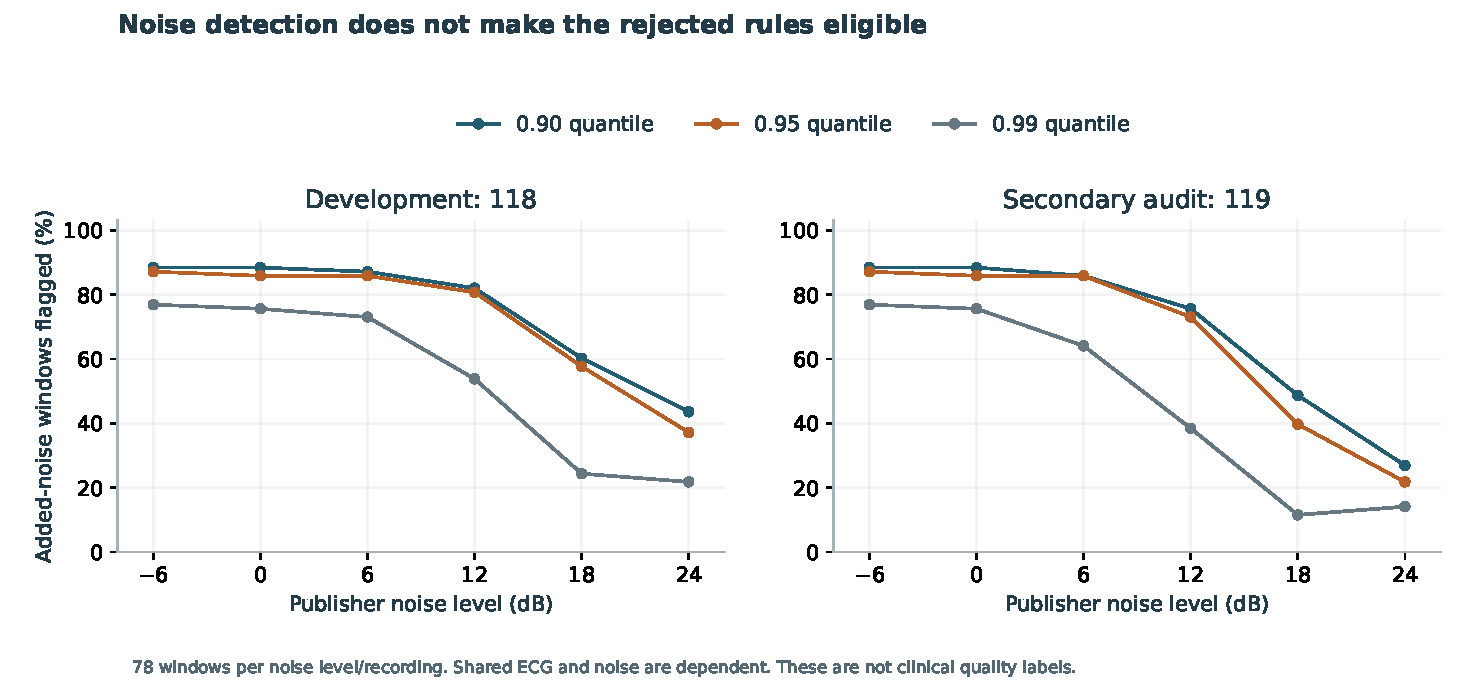
\includegraphics[width=\linewidth]{images/noise_detection_tradeoff.pdf}\end{center}
\captionof{figure}{The complete six-level noise diagnostic uses the same underlying recording and noise across variants. Lines connect fixed stress levels for readability, without an interpolated performance claim. Stronger detection at lower source SNR does not repair the source-clean rejection failures. All plotted candidates were rejected during development; none is selected from this figure.}

\textbf{Evidence limit.} This is one development source recording and one later source recording. Windows share physiology, source noise and time structure. No random-window bootstrap, population confidence interval, p-value, natural prevalence or effective independent subject count is claimed. The study does not distinguish actual recording devices or evaluate downstream diagnostic mistakes.
\newpage
\section*{4. Numerical sensitivity and an implementation exercise}
The authored gain/offset transform $y=2x+0.5$ mV leaves both feature definitions invariant algebraically: centering removes the additive constant, and numerator/denominator energies share the squared gain. All scored candidate decisions are unchanged in both recordings within the fixed feature tolerance.

A separate authored quantization transform rounds to 0.02 mV using ties-to-even. It is a numerical sensitivity, not a measured device change. The number of changed decisions among each candidate's 618 scored windows is:
\begin{center}\begin{tabular}{@{}lrr@{}}\toprule
Rejected candidate quantile & Development flips & Later flips\\\midrule
0.90 & 11 & 4 \\
0.95 & 3 & 0 \\
0.99 & 3 & 0 \\
\bottomrule\end{tabular}\end{center}

The fallback changes no decision. These counts do not estimate a device error rate or validate the chosen step size. Complete clean/noise strata and both transformations remain in the exports; no threshold is retuned after perturbation.

\begin{center}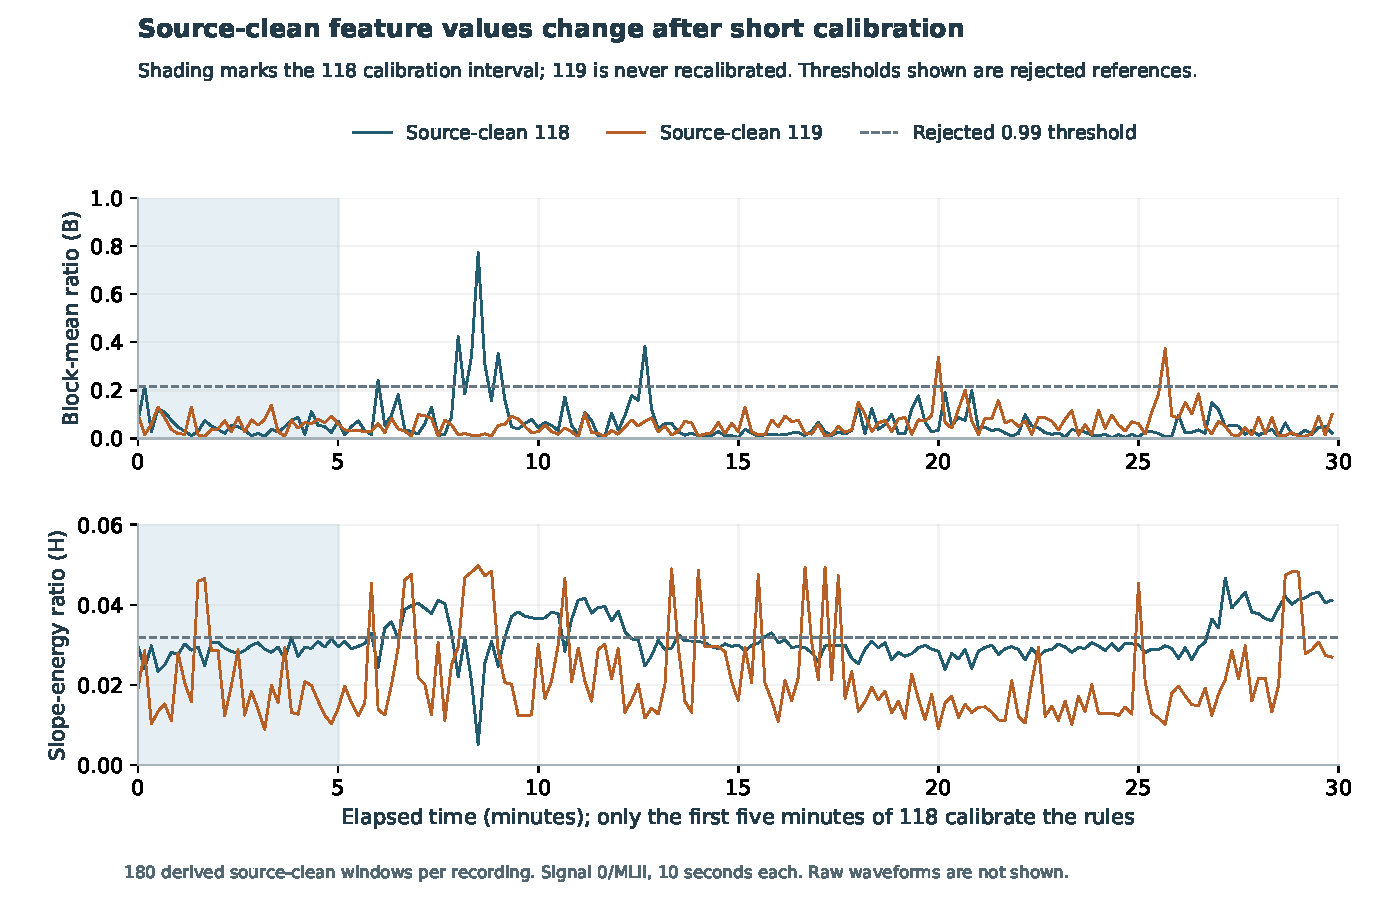
\includegraphics[width=.89\linewidth]{images/source_clean_feature_drift.pdf}\end{center}
\captionof{figure}{Derived source-clean features reveal why a short calibration can miss later variation. Only recording 118's shaded initial period calibrates thresholds. Dashed lines show the rejected 0.99-quantile references, not the selected fallback. The plot contains per-window features, without raw waveforms or clinical rhythm labels. Visual variation does not identify its physiological or recording cause.}

\textbf{Exercise.} The offline CLI accepts a single-column mV CSV with exactly one complete window and the explicit 360 Hz rate. It returns features, the frozen demonstration flag and threshold reasons; its clinical quality judgment is unavailable. The authored alternating-value fixture has analytical values $B=0$, $H=4$. Flat/nonfinite/incorrect-length input returns unavailable. An optional diagnostic mode clearly identifies an already rejected candidate. This is an implementation and evidence-review exercise, without instructions to suppress clinical alarms.
\newpage
\section*{5. Independent checks, reproducibility and next evidence}
Original-record checks use an independently installed WFDB reader rather than the feature generator's decoder. Scalar sums and grouped means independently reconstruct the derived feature projection; SQL verifies complete keys, source roles and recording separation. Each recording's 3,888 feature values pass 10,391 source-feature/key conditions. A separate checker reconstructs thresholds, nearest ranks, feasibility, tie-breaks, confusion counts, exact fractional rates and perturbation flips from the observation exports: 45,028 development and 45,029 later conditions. These are finite implementation checks, not independent patients or a clinical correctness guarantee.

The suite contains 27 finite test methods, including additional parameterized cases for native signed decoding, missing/truncated inputs, schedule boundaries, analytical waveforms, invariant transforms, rank ties, selection constraints, duplicate controls, recording IDs and unavailable CLI input. The figures pass 765 source-value, 1,572 actual SVG-coordinate and 9 export-hash checks. Numerical checks are paired with separate visual inspection; source validity cannot be inferred from an attractive chart.

\textbf{Replay boundary.} The public reproduction command uses a full-history clone, verifies the committed pre-later dependencies, reruns tests and analysis into separate paths, and compares deterministic predictions, metrics, strata, sensitivities and selection documents. It verifies unchanged original public files. It does not retrieve source waveforms or pretend derived-input replay is a new raw-waveform validation. Re-extraction requires the separately preserved originals and optional WFDB environment. Execution timestamps/runtimes are observations, not deterministic output targets. One initial development invocation's runtime was not retained; both identical primary result outputs remain in the task trace, as the execution note discloses.

\textbf{Practical next evidence.} Keep the failed gates out of operational use. An expanded study would need multiple independent participants, representative recording conditions and device identities, expert acceptability labels that include arrhythmias, and an independently justified cost of rejection. Fit and validate any replacement only after fixing those criteria and a fresh protected evaluation. This small benchmark neither establishes a new quality index nor shows a clinical safety improvement.

\textbf{Prior work and attribution.} Noise stress testing and ECG quality indices predate this study. Existing work also warns that physiological differences can affect quality-index behavior. Primary references and source rights:
\begin{enumerate}\setlength{\itemsep}{1pt}
\item Moody, Muldrow and Mark (1984), \textit{A noise stress test for arrhythmia detectors}; Moody and Mark (2001), \textit{The impact of the MIT-BIH Arrhythmia Database}. Sources: \url{https://physionet.org/content/nstdb/1.0.0/} and \url{https://physionet.org/content/mitdb/1.0.0/}.
\item Publisher NST generator, signal and header specifications: \url{https://physionet.org/physiotools/wag/nst-1.htm}, with linked native-format documentation. ODC Attribution 1.0: \url{https://opendatacommons.org/licenses/by/1-0/}. Dataset license pages are preserved in the source receipts.
\item Clifford et al. (2012), \textit{Signal quality indices and data fusion for determining clinical acceptability of electrocardiograms}, \url{https://doi.org/10.1088/0967-3334/33/9/1419}.
\item Daluwatte et al. (2016), \textit{Assessing ECG signal quality indices to discriminate ECGs with artefacts from pathologically different arrhythmic ECGs}, \url{https://pmc.ncbi.nlm.nih.gov/articles/PMC4975422/}. PhysioNet platform attribution is linked in DATA\_RIGHTS.md and the preserved source descriptions.
\end{enumerate}
\textbf{Publication scope.} Independent, not peer reviewed. Public derived benchmark evidence only; separate formal-publication projects, including Azure optimization, remain private. No clinical deployment, adoption, patient benefit or realized financial impact is established.
\end{document}
